%%%%%%%%%%%%%%%%%%%%%%%%%%%%%%%%%%%%%%%%%%%%%%%%%%%%%%%%%%%%%%%
%%  Versão final do IEEExplore
%%%%%%%%%%%%%%%%%%%%%%%%%%%%%%%%%%%%%%%%%%%%%%%%%%%%%%%%%%%%%%%

%\documentclass[10pt, conference, compsocconf]{IEEEtran}
\documentclass[a4paper]{sbgames}               

\usepackage{times}
\usepackage{graphicx}
\usepackage{hyperref}
\usepackage{amsmath,amssymb,amsthm,siunitx}
\usepackage[brazil,american]{babel}
\usepackage[utf8]{inputenc}

%% use this for zero \parindent and non-zero \parskip, intelligently.
\usepackage{parskip}

%% the 'caption' package provides a nicer-looking replacement
%\usepackage[labelfont=bf,textfont=it]{caption}

\usepackage{url}

\begin{document}

%% Paper title.
\title{Snake em Assembly MIPS}


% \author{\IEEEauthorblockN{Autor1, Autor2, and Autor3}
% \IEEEauthorblockA{Dept. of Computer Science\\
% University of Brasilia\\ Brasilia, Brazil\\
% Email: \{autor1, autor2\}@gmail.com autor3@hotmail.com}
% }

 \author{ Gabriel Lobão 
         \hspace{28pt} Gabriel Nunes \hspace{28pt} Mikael Mello\\
         \vspace{0pt} \\
         {Universidade de Brasília, Dept. de Ciência da Computação, Brasil} }
        
 \contactinfo{autor1@gmail.com \\ autor2@hotmail.br }



%\teaser{
%  \includegraphics[width=\linewidth]{sample.pdf}
%  (a)\hspace{150pt} (b) \hspace{150pt}   (c)
%  \caption{(a) Guitar Hero III screen; (b) DE2-35 Kit on top of PlayStation 2; (c) Grybot}
%  \label{fig:01}
%}


% make the title area
\maketitle

% Abstract section.
\begin{abstract}

Este trabalho apresenta o desenvolvimento de  um jogo famoso conhecido como Snake ou no Brasil como "o jogo da cobrinha". O jogo se trata de uma cobra que é controlada pelo jogador que busca comida e a medida que ela pega a comida ela cresce. Nesta versão o jogador perde quando a cobra colide nela mesma ou no limite das laterais da arena do jogo. O jogo foi desenvolvido na linguagem MIPS32 Assembly com auxílio da IDE MARS (\textit{MIPS Assembler Runtime Simulator}).

\begin{figure}[htb]
  \begin{center}
   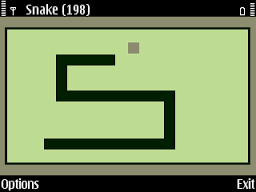
\includegraphics[width=1.0\linewidth]{./Figures/snakegoogle.png}
  \end{center}
  \caption{Imagem de um \textit{Snake} retirada da Internet}
  \label{fig:03}
\end{figure}

\end{abstract}

%% Keywords that describe your work.
\keywords{Robot, Guitar Hero, FPGA, Artificial Intelligence}
% \begin{IEEEkeywords}
% Jogos; Processador MIPS; FPGA;
% \end{IEEEkeywords}


\section{Introdução}
\label{sec:introducao}

	A criação do jogo da cobrinha representa um grande desafio lógico pela dificuldade de implementar um algoritmo conciso, sem falhas e rápido. Tal projeto necessita ser visto com cautela pois é um software extenso de uso comum, então está sujeito à \textit{bugs} causados por mau uso ou execução e também causados por falhas do próprio simulador MARS. 
    
	A linguagem Assembly MIPS32, na qual o programa foi escrito, apresenta certas limitações em seu conjunto de instruções pelo seu baixo nível, configurando um desafio a mais em programar um jogo da cobrinha que seja divertido, desafiador e cativante.  Elementos como cores, sons, dificuldade crescente e número limite de vidas até o fim de jogo, são propositalmente inseridos com o intuito de tornar o programa chamativo ao usuário e também estimular a competitividade.

	O projeto visa a prática da implementação em Assembly MIPS32 e o desenvolvimento de competências como raciocínio lógico e o trabalho em equipe, visa também o aprendizado do grupo estudantil em relação ao processador MIPS de 32 bits, como funciona seu banco de registradores, suas rotinas, acesso à memoria, pilha de dados, etc.

    

\section{Metodologia}
\label{sec:Metodologia}

Este jogo foi desenvolvido usando a linguagem Assembly MIPS32, explicada na seção \ref{sec:MIPS}, juntamente com uma versão modificada do simulador MARS, explicado na seção \ref{sec:Mars}, onde algumas pequenas mudanças estão presentes como por exemplo [dizer as principais mudanças depois que o Lamar responder o \textit{e-mail} falando quais elas são], assim como o uso de um gerenciador de exceções especial, usado para imprimir caracteres no \textit{Bitmap Display}.

Também foi utilizado um pequeno programa escrito na linguagem C com o objetivo de transformar uma imagem no formato bitmap de 256 bits em um arquivo binário contendo apenas os \textit{bytes} da imagem, retirando o cabeçalho de um arquivo bitmap normal, por exemplo, e realizando outras pequenas tarefas.

Todo o histórico de alterações nos arquivos do projeto e o próprio código-fonte do mesmo podem ser encontrados no repositório público do Github sob o nome "snake-assembly-mips", encontrado na URL \url{https://github.com/MikaelMello/snake-assembly-mips}.

\subsection{Arquitetura MIPS}{
\label{sec:MIPS}
Antes de mais nada é importante esclarecer o que é uma arquitetura. Arquitetura é a parte do processador visível ao usuário e nela contém tanto o conjunto de instruções quanto a forma de endereçar os dados. 

A arquitetura MIPS \cite{patterson2005organizaccao} foi desenvolvida por John Hennessy em 1981, porém sua empresa foi criada apenas em 1984. Sua arquitetura é baseada em registradores para operações lógicas e aritméticas. Existem outros tipos: alguns que se baseiam em pilha, outros em acumuladores, entre outros. A arquitetura MIPS foi além do que se esperava. Hoje em dia, vários cursos estudam essa arquitetura e diversos projetos de arquitetura de processadores se basearam na MIPS. É também importante citar que ela é uma arquitetura de microprocessadores RISC, isto é, ele possui um conjunto reduzido de instruções. Suas instruções possuem um tempo de execução muito próximo uma da outra. Isso se deu por conta de uma grande novidade dos processadores MIPS, que foi o uso de pipelines, que tem como função de dividir a tarefa de execução de uma instrução em diversas etapas.

O datapath do processador MIPS é constituído de um mecanismo para ir a próxima instrução e uma memória de instruções. Após isso, há um mecanismo de controle das operações, tais como ler ou não algo do banco de registradores, ou um comando de jump, ou as operações lógica/aritméticas, entre outros. Além disso, há o banco de registradores como já citado, a memória de dados, e a ULA (Unidade Lógica e Aritmética), que como o seu nome já descreve administra as operações lógica/aritméticas.

\begin{figure}[htb]
  \begin{center}
   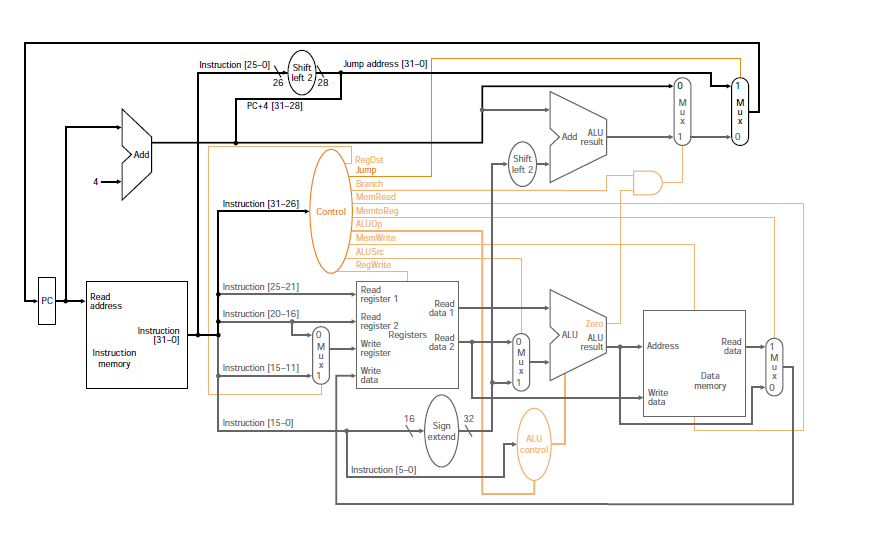
\includegraphics[width=1.0\linewidth]{./Figures/Datapath.png}
  \caption{Datapath do MIPS e amostra da execução de tarefas por meio de \textit{pipeline}}
  \end{center}
  \label{fig:02}
\end{figure}

\subsection{Simulador/Montador MARS}{
\label{sec:Mars}
O Mars \textit{MIPS Assembler and Runtime Simulator} \cite{Mars1} é um simulador desenvolvido pela \textit{Missouri State University}. Ele tem a função de ser um simulador e também um montador para execução de programas de linguagem Assembly MIPS. 

\begin{figure}[htb]
  \begin{center}
   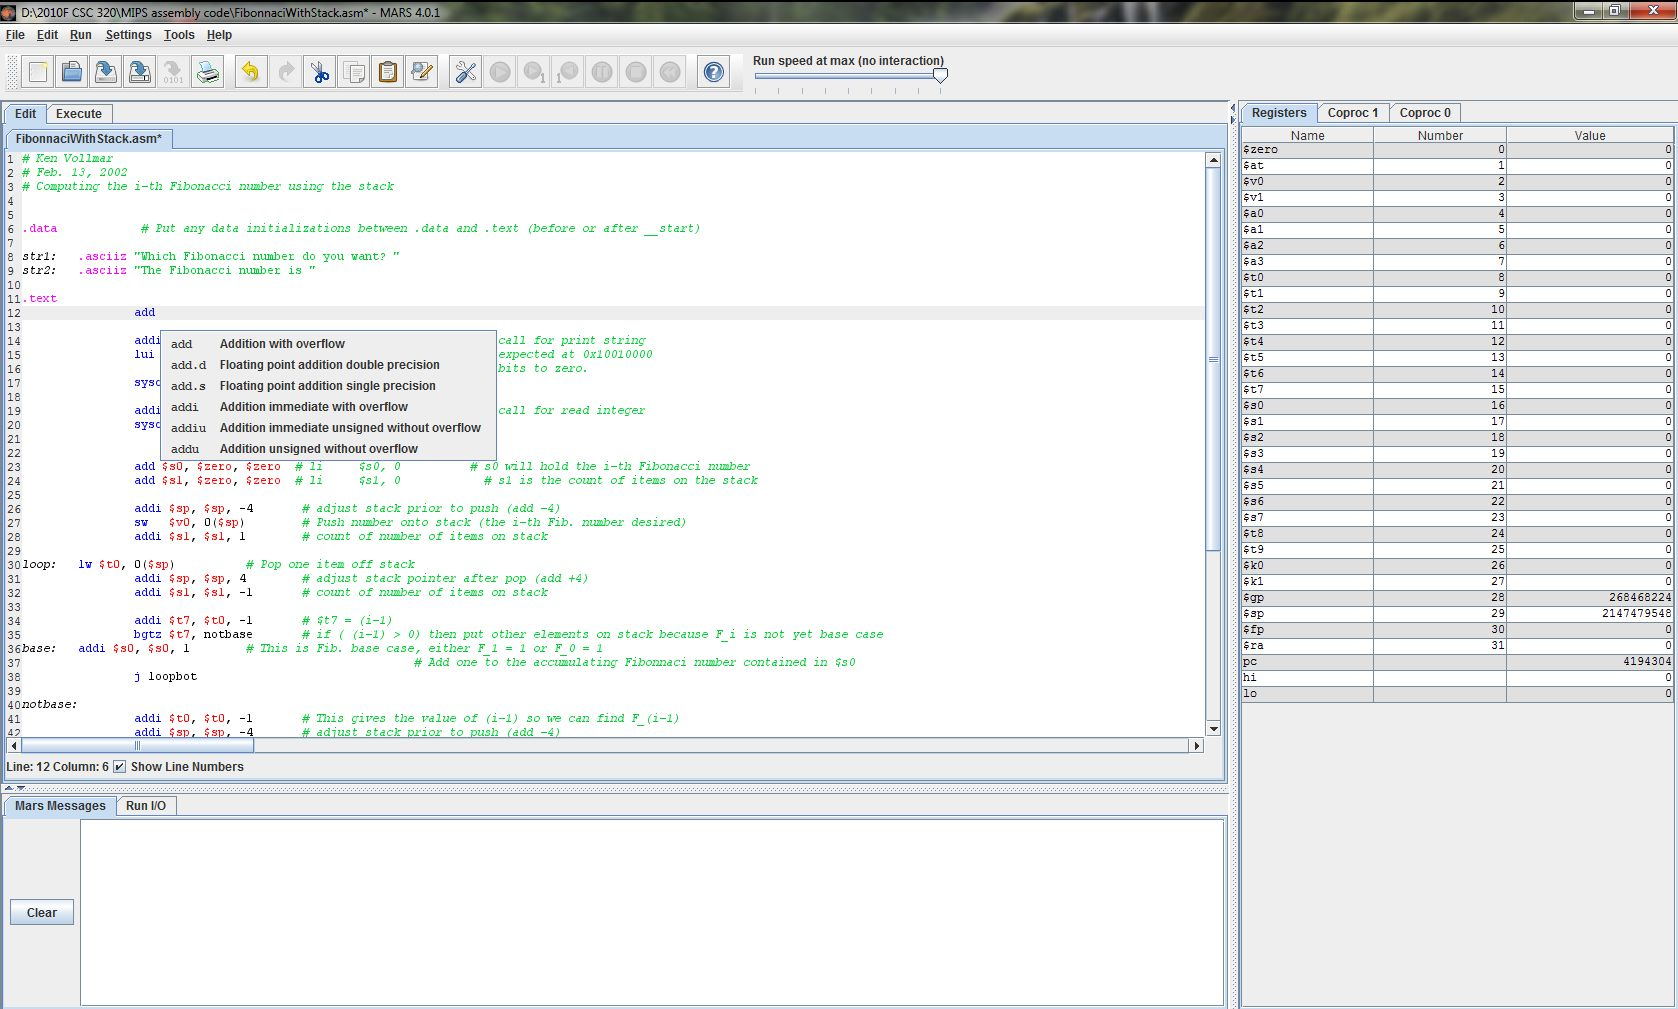
\includegraphics[width=1.0\linewidth]{./Figures/marscode.jpg}
  \end{center}
  \caption{Exemplo de uma janela do MARS}
  \label{fig:07}
\end{figure}

Esse simulador possui diversas ferramentas com o objetivo de auxiliar o programador a melhor simular um processador MIPS. Neste projeto são usados ambos \textit{Bitmap Display} e \textit{Keyboard and Display MMIO Simulator}.

O \textit{Bitmap Display} tem como função mostrar na tela uma imagem por meio de uma memória mapeada onde cada pixel equivale a uma certa quantidade de \textit{bytes}, definida pelo programador. Esta ferramenta foi fundamental para o desenvolvimento do jogo uma vez que o usuário necessita de acompanhar a posição atual da cobrinha além de obter outras informações a respeito do estado atual do jogo.

O \textit{Keyboard and Display MMIO Simulator} tem a função de simular o teclado do computador na tela. Ele pode ser usado tanto como ferramenta de entrada, onde o usuário digita em um certo campo, como também de saída, onde podem ser impressas mensagens específicas. Esta também foi uma ferramenta essencial no trabalho para tornar possível o movimento automático da cobra quando o usuário não pressionava nenhuma tecla (ou alguma inválida) assim como ler as teclas válidas de entrada do usuário.

\begin{figure}[htb]
  \begin{center}
   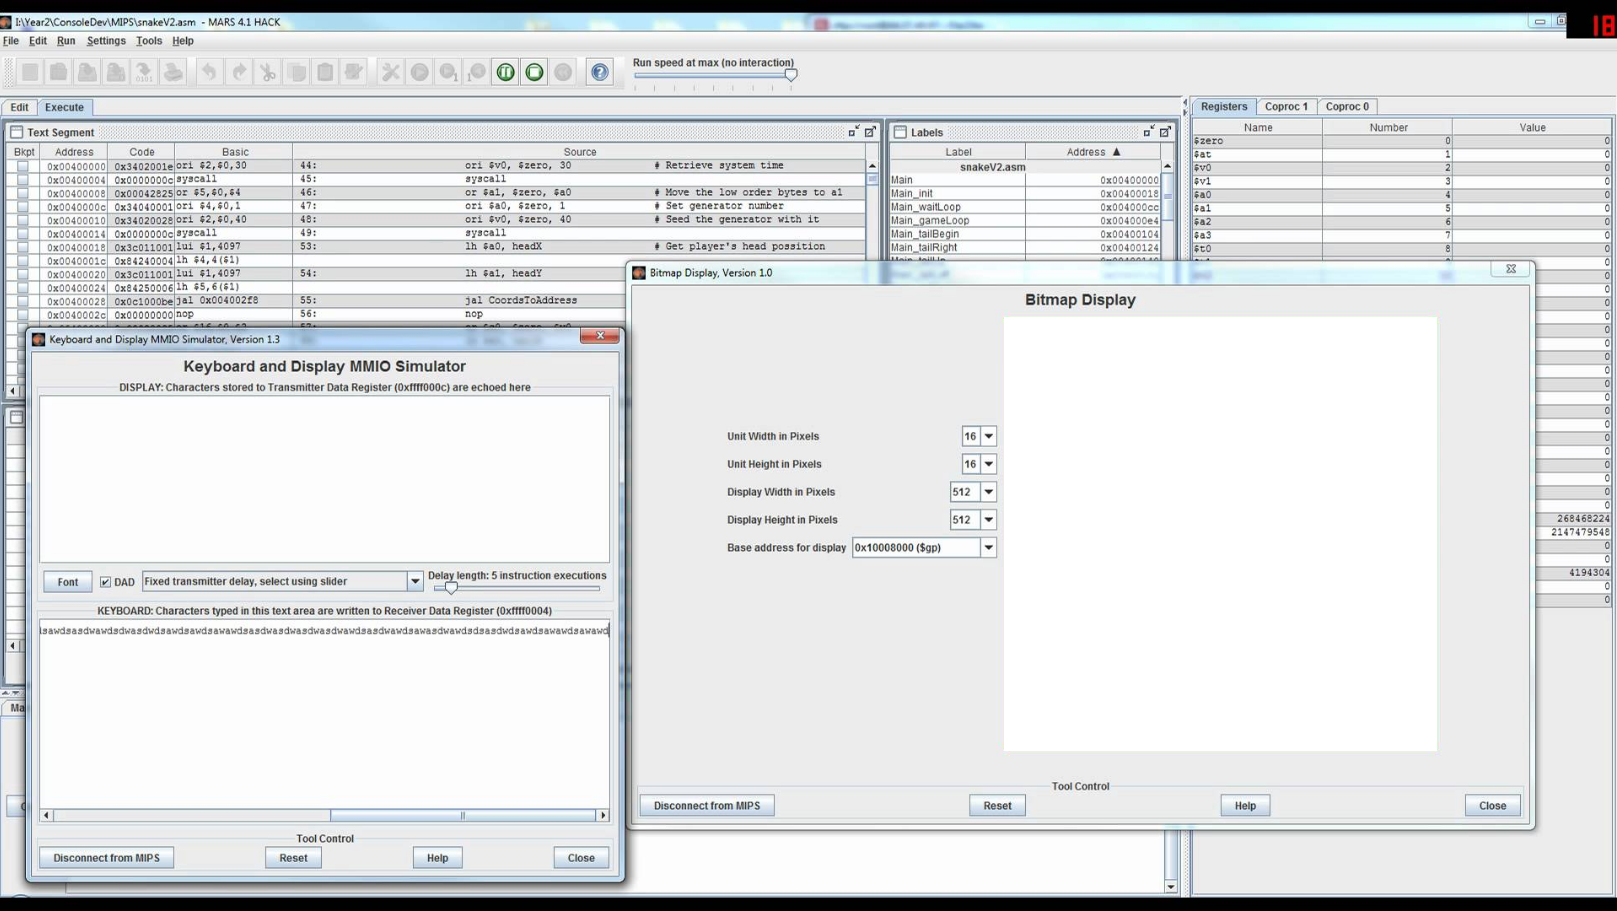
\includegraphics[width=1.0\linewidth]{./Figures/marstools.png}
  \end{center}
  \caption{Janelas de ambas ferramentas usadas}
  \label{fig:08}
\end{figure}


\subsection{Desenvolvimento}
\label{sec:Desenvolvimento}

Nas primeiras etapas do projeto, foi desenvolvido o preenchimento da tela de fundo com uma cor escura e logo depois uma cor rosa em uma porção menor da tela, sendo esta a arena do jogo por onde a cobra anda. 

A estrutura principal do jogo trata-se de um laço de repetição infinito onde a cada iteração são carregadas informações da memória e da entrada do usuário, realizando as ações mais apropriadas à situação.

Logo após, foi implementado o início do que seria no futuro o sistema de movimento da cobra. Neste estágio do desenvolvimento, o corpo era estático e apenas a cabeça da cobra era movida, movimento este realizado ao colorir a posição atual da cabeça da cobra com a cor do corpo dela (preto) e logo depois colorir a próxima posição da cabeça de verde. Para facilitar, na seção de dados estão guardadas as posições $x$ e $y$ (como em um plano cartesiano) da cabeça e do último pedaço do corpo da cobra. Neste plano cartesiano, a origem é o canto superior esquerdo da tela rosa.

De modo a deixar o sistema de movimento completamente funcional, é alocada na \textit{stack} uma quantidade $x = n-1$ de \textit{words}, sendo $n$ o tamanho atual da cobra. Em cada \textit{word} está contido um número de 1 a 4 que significam a direção da parte atual do corpo da cobra para a próxima parte, seguindo-se até a cabeça. Estes números 1, 2, 3 e 4 indicam norte, oeste, sul, leste, respectivamente. Assim, a cada iteração do laço principal do jogo, são atualizadas as posições da cabeça e da cauda da cobra. A entrada do usuário, neste estágio, é carregada por meio de uma chamada do sistema (\textit{syscall}) e por isso o movimento ainda não é executado automaticamente.

Com o sistema de movimento corretamente implementado, iniciou-se o desenvolvimento do sistema de crescimento e colisão. Assim como a cabeça e a cauda da cobra, a posição da comida também é guardada na memória, assim a cada iteração é verificado se a posição da cabeça é a mesma da comida, caso seja, a cauda atual não é deletada nesta iteração e por isso a cobra cresce uma unidade de tamanho. No sistema de colisão, em cada iteração é checado se ambos $x$ ou $y$ são negativos ou maiores que o limite, caso sejam, o jogo chega ao seu fim, pois neste estágio as vidas ainda não foram implementadas. Também deve-se checar se a cobra não entra em colisão consigo mesma, por isto é alocado na memória um espaço de 3800 \textit{bytes}, uma matriz de dimensões 304x200, o tamanho da arena do jogo. Nesta matriz, todos os espaços estão preenchidos com 0, exceto aqueles em que a cobra se encontra, onde o valor encontrado é 1. Deste modo, basta apenas checar se a nova posição da cabeça da cobra, nesta matriz, é 0 ou 1, caso seja 1, o jogo acaba.

Em seguida, implementar a pontuação, as vidas e os efeitos sonoros foi uma tarefa simples. Ambas as vidas e a pontuação são guardadas na memória, as vidas são atualizadas somente no caso de uma colisão, verificadas com o sistema acima. A pontuação é calculada da seguinte forma, sendo $p$ a pontuação atual e $t$ o tamanho atual da cobra, a nova pontuação é calculada como $p = p + t$, sendo ela atualizada apenas na ocasião de crescimento. Os efeitos sonoros são simples chamadas de sistemas usando o sistema MIDI. Para o movimento automático, bastou trocar as chamadas de sistema para o uso da ferramenta  \textit{Keyboard \& Display MMIO} e a adição de uma chamada de sistema para pausar a execução do \textit{loop} por alguns milisegundos, pausa esta que é diminuída conforme o usuário avança no jogo, de modo a aumentar a dificuldade.

O desafio do projeto foi carregar imagens customizadas no \textit{Bitmap Display}. Como o MARS trabalha apenas com \textit{bytes} que representam cores, não é possível carregar imagens diretamente. Deste modo faz-se necessário a conversão de um arquivo de imagem para um binário contendo apenas os \textit{bytes} das cores. Após uma pesquisa extensiva, não foi encontrado nenhum programa que fazia esta conversão perfeitamente, assim, para o projeto, foi desenvolvido um pequena programa em C, já descrito na seção \ref{sec:Metodologia}. Deste modo, foram inseridas imagens para indicar as vidas restantes, o fim do jogo, a contagem regressiva para o início do jogo e o painel onde estão presentes as informações sobre a pontuação atual e o tamanho da cobra.

Por fim, foram utilizadas chamadas de sistema customizadas, encontradas no arquivo SYSTEMv52.s presente no repositório do Github, com o principal objetivo de imprimir na tela a pontuação e o tamanho da cobra atuais, sendo eles atualizados toda vez que o sistema de crescimento é acionado.

\section{Resultados Obtidos}
\label{sec:Resultados}
Ao final do projeto, está desenvolvido um jogo \textit{Snake} funcional, para jogá-lo basta abri-lo e montá-lo no MARS conforme instruções presentes no repositório do \textit{Github}.

Ao rodar, para mudar a direção da cobra basta pressionar as teclas W, A, S ou D, caso a nova direção seja diretamente contrária à atual, seu novo movimento será ignorado e a cobra seguirá na direção anterior.

No início do jogo e a cada vida perdida, o usuário verá uma tela de preparação contando com até 4 segundos (incluindo-se a tela "GO", vide figura \ref{fig:04}) para a cobra começar a andar automaticamente.

\begin{figure}[htb]
  \begin{center}
   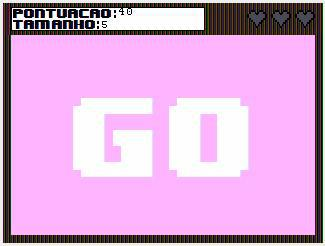
\includegraphics[width=1.0\linewidth]{./Figures/go.jpg}
  \caption{Tela prestes a iniciar o jogo}
  \end{center}
  \label{fig:04}
\end{figure}

Depois do fim da contagem regressiva, o usuário, controlando a cobra com W, A, S ou D, deve comer uma maçã, representada pelo quadrado vermelho, indo até o quadrado onde ela está. Sua pontuação e seu tamanho são atualizados a cada vez que comer uma maçã, exceto na primeira vez, onde apenas o tamanho é acrescentado. Caso o usuário ande com a cobra até alguma das quatro bordas ou faça a cobra "comer" o próprio corpo, ele perde uma vida, um efeito sonoro é tocado e o jogo é reiniciado, .

\begin{figure}[htb]
  \begin{center}
   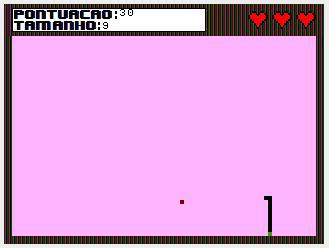
\includegraphics[width=1.0\linewidth]{./Figures/snake1.jpg}
  \caption{Usuário prestes a perder uma vida}
  \end{center}
  \label{fig:05}
\end{figure}

Se não houver nenhuma vida restante, o jogo acaba, toca-se uma música específica e é mostrada uma tela escrito \textit{GAME OVER},

\begin{figure}[htb]
  \begin{center}
   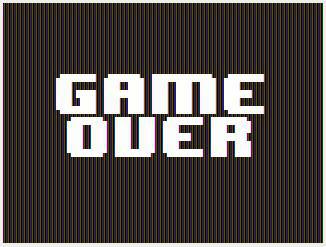
\includegraphics[width=1.0\linewidth]{./Figures/gameover.jpg}
  \caption{Tela de fim de jogo.}
  \end{center}
  \label{fig:06}
\end{figure}

\section{Conclusão}
\label{sec:Conclusao}
Neste projeto, por ter sido realizado em uma linguagem de baixo-nível, foram enfrentadas várias dificuldades que, apesar de poderem ter sido evitadas usando-se outras linguagens de programação, são fundamentais para entender os aspectos básicos da computação, conhecimentos estes necessários para qualquer bom cientista da computação.

Além da programação em baixo-nível, houve a necessidade de aprender sobre a estrutura geral de um jogo simples, o que pode vir a ser útil em futuros projetos relacionados, assim como também houve o treino da escrita e formatação de um artigo científico em LaTeX, necessário para a formação acadêmica.

Houve também a aplicação do método científico na prática, em que diante de cada problema lógico eram estabelecidas hipóteses a serem avaliadas e testadas afim de selecionar a melhor opção para resolver dito problema.

%{\bf Acknowledgments}
%[Blind Review]

%\newcommand{\BIBdecl}{\setlength{\itemsep}{-0.5 em}}
%\bibliographystyle{IEEEtran}
\bibliographystyle{sbgames}
\bibliography{bibliography}

\end{document}
